\documentclass[12pt,letterpaper]{article}
\usepackage[utf8]{inputenc}
\usepackage{amsmath}
\usepackage{amsfonts}
\usepackage{amssymb}
\usepackage{amsthm}
\usepackage{graphicx}

\usepackage{hyperref}
\hypersetup{
    colorlinks=true,
    linkcolor=blue,
    filecolor=magenta,      
    urlcolor=cyan,
}
\urlstyle{same}

\usepackage{tabularx}
\usepackage[left=2cm,right=2cm,top=2cm,bottom=2cm]{geometry}
\usepackage{fancyhdr}
\usepackage{multicol}
\usepackage{multirow,array}
\usepackage{newtxtext,newtxmath}
\usepackage{relsize}
\usepackage{lastpage}
\usepackage{enumitem}
\usepackage{adjustbox}
\newcolumntype{Y}{>{\centering\arraybackslash}X}
	\setenumerate[1]{label={\bf Q\theenumi: ~}}
	\setenumerate[2]{label={\bf \theenumii: ~}}
\pagestyle{fancy}
\fancyhf{}
\lhead{BHCC Mat-181}
\rhead{\textsc{Confidence Intervals}}
\rfoot{Page \thepage ~of \pageref*{LastPage}}



\begin{document}
The random variable $Z$ is normally distributed such that $\mu=0$ and $\sigma=1$. It has the following probability density function.
$$\phi(z) = \cfrac{e^{-z^2/2}}{\sqrt{2\pi}} $$
This function gives us the bell-shaped curve we are accustomed to.
\begin{center}
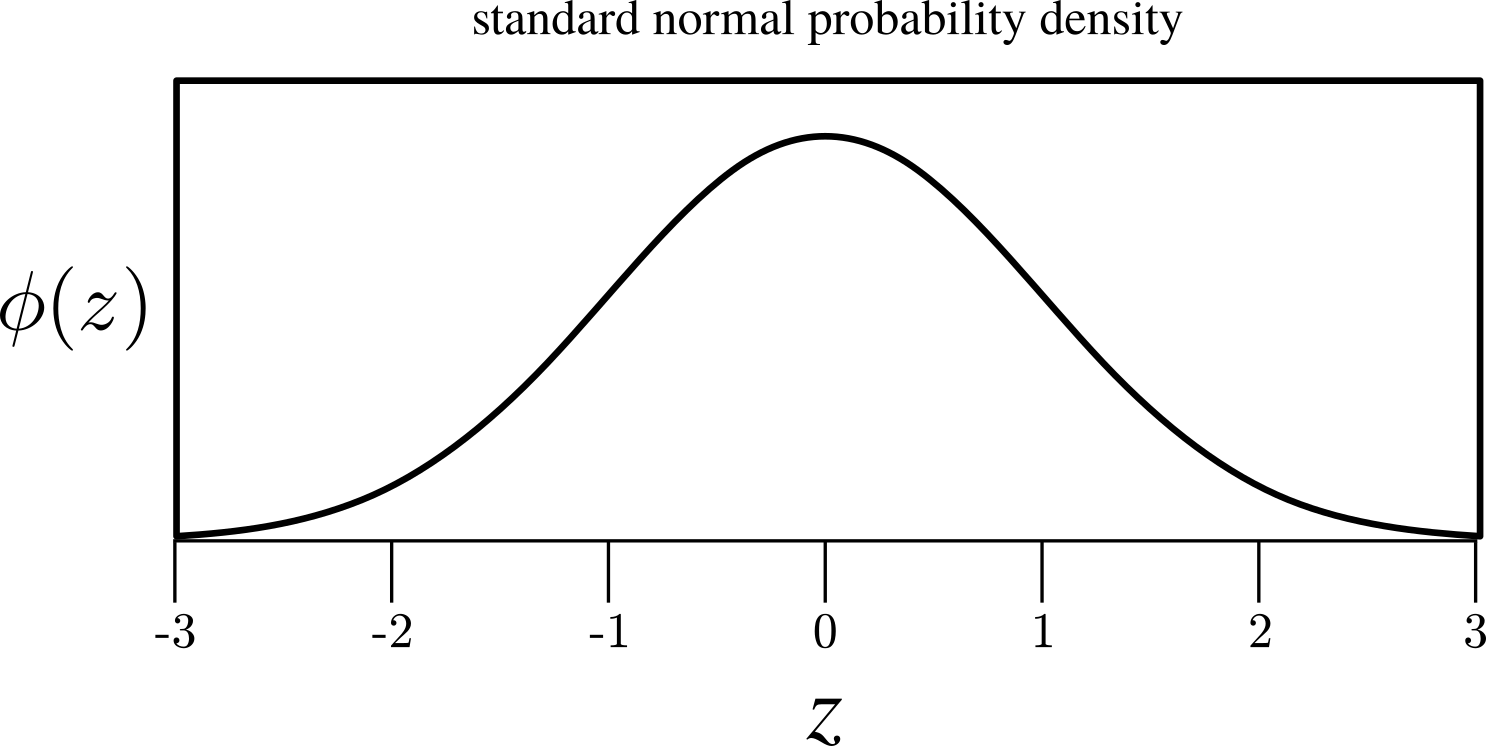
\includegraphics[scale=.7]{phi.png}
\end{center}
To determine the probability that $Z$ is less than $z_0$, we find the area under the curve from $-\infty$ to $z_0$.
\begin{center}
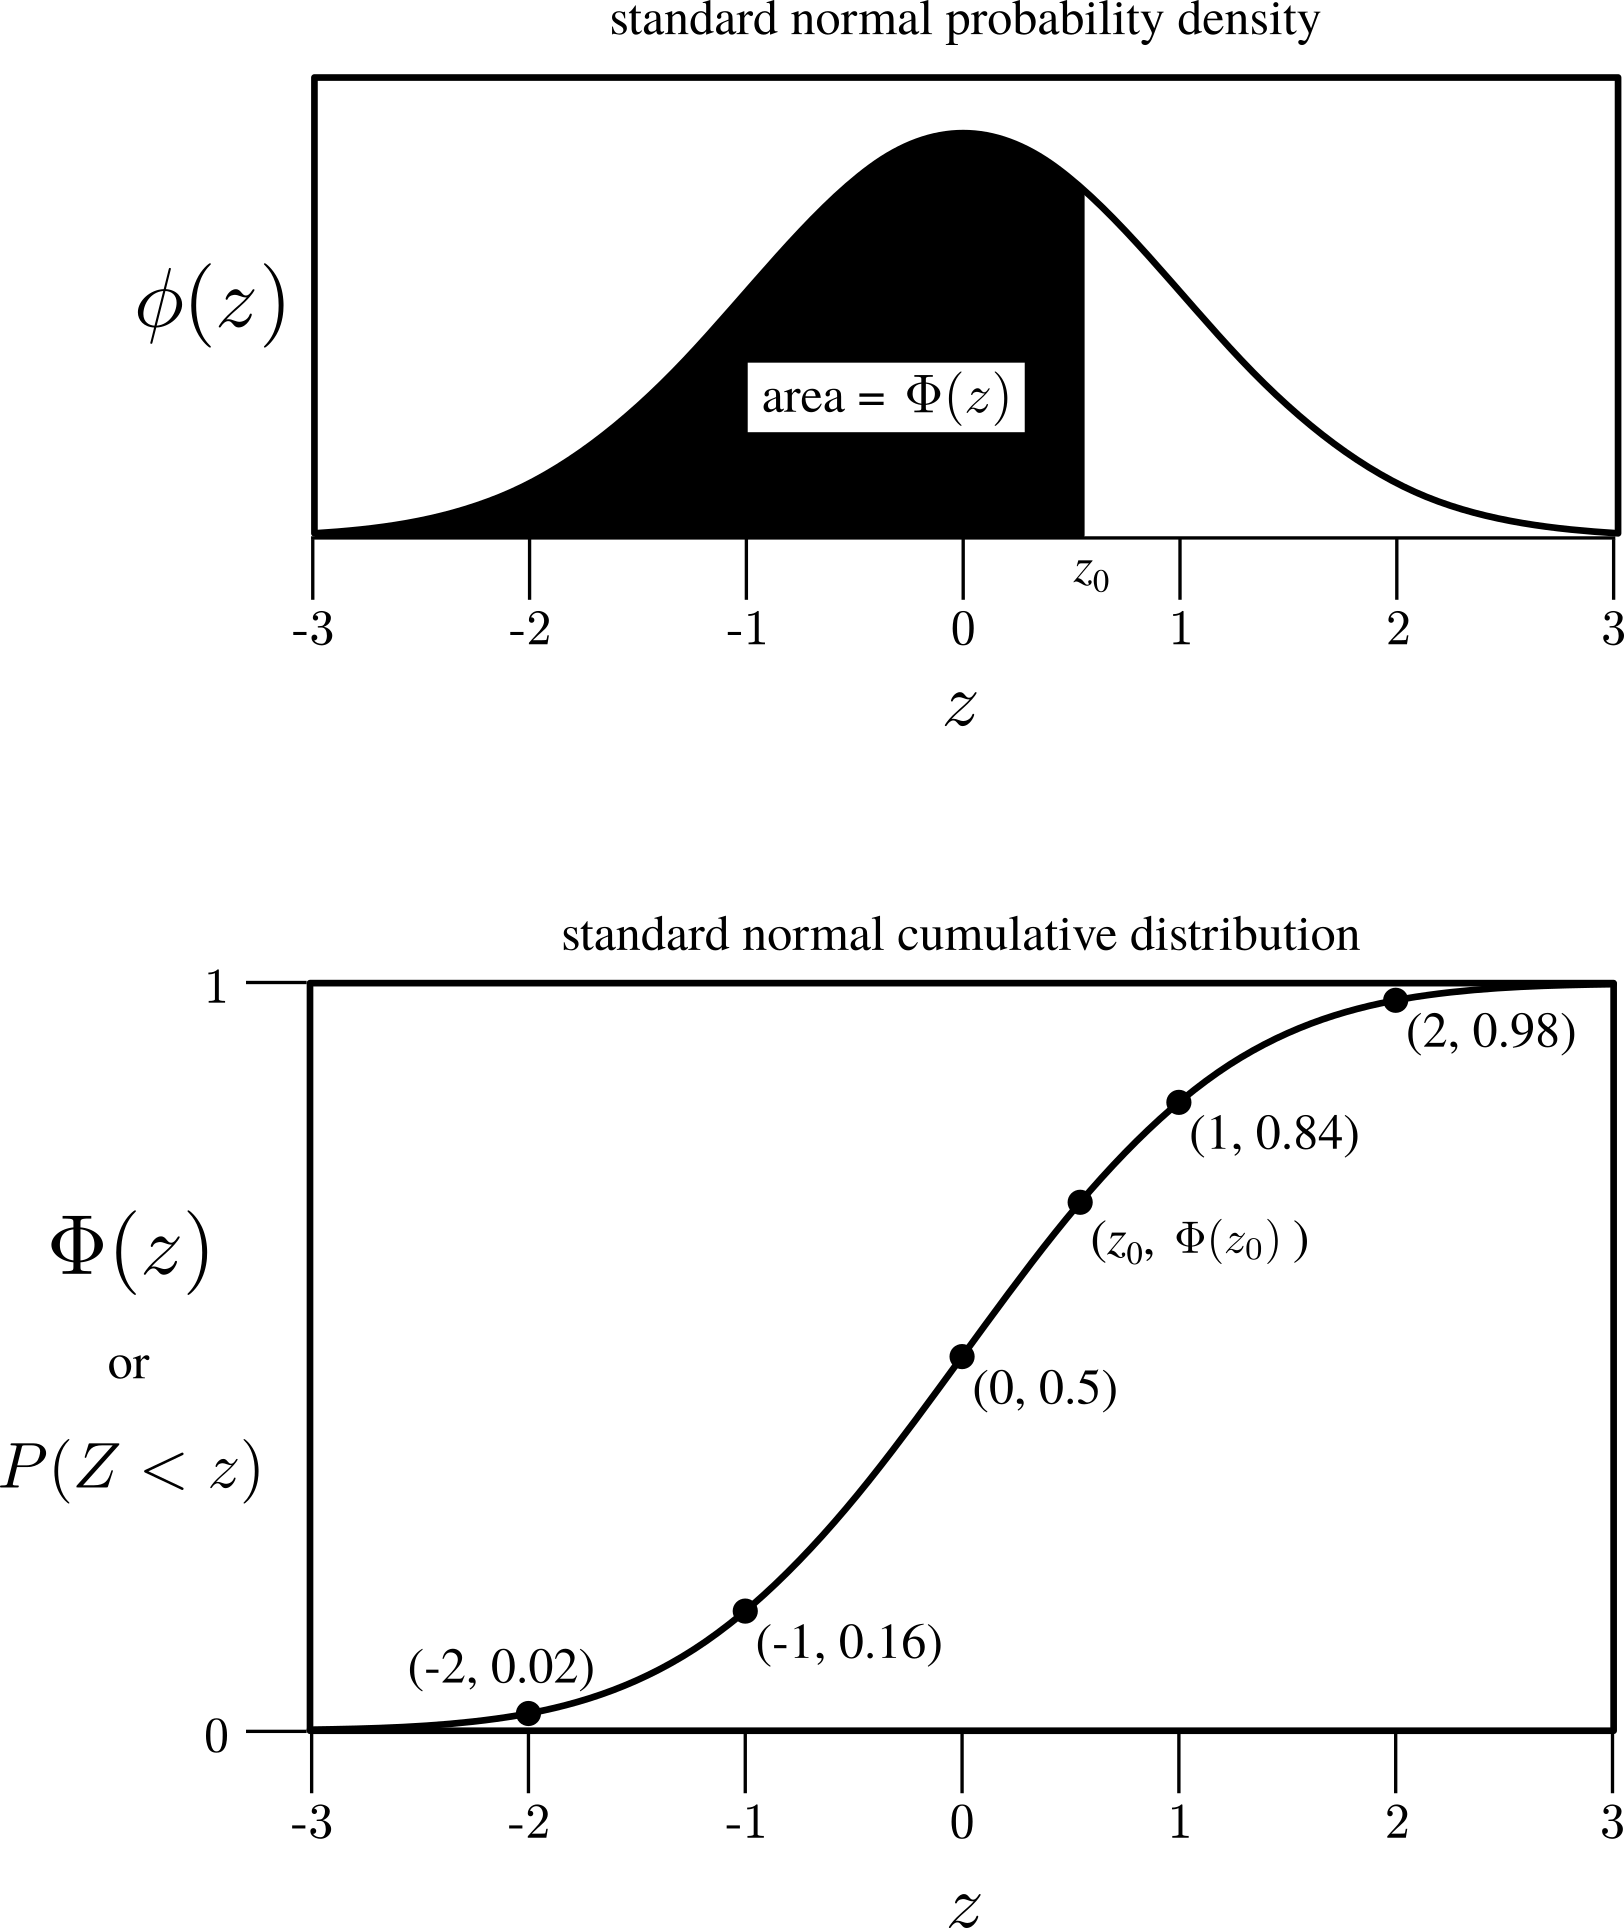
\includegraphics[scale=.7]{both.png}
\end{center}

Notice the notation. We use a lower-case phi, $\phi$, for the density function and an upper-case phi ,$\Phi$, for the cumulative function.

The standard normal table gives precise values of $\Phi$ as a function of $z$. 
\newpage
\begin{center}
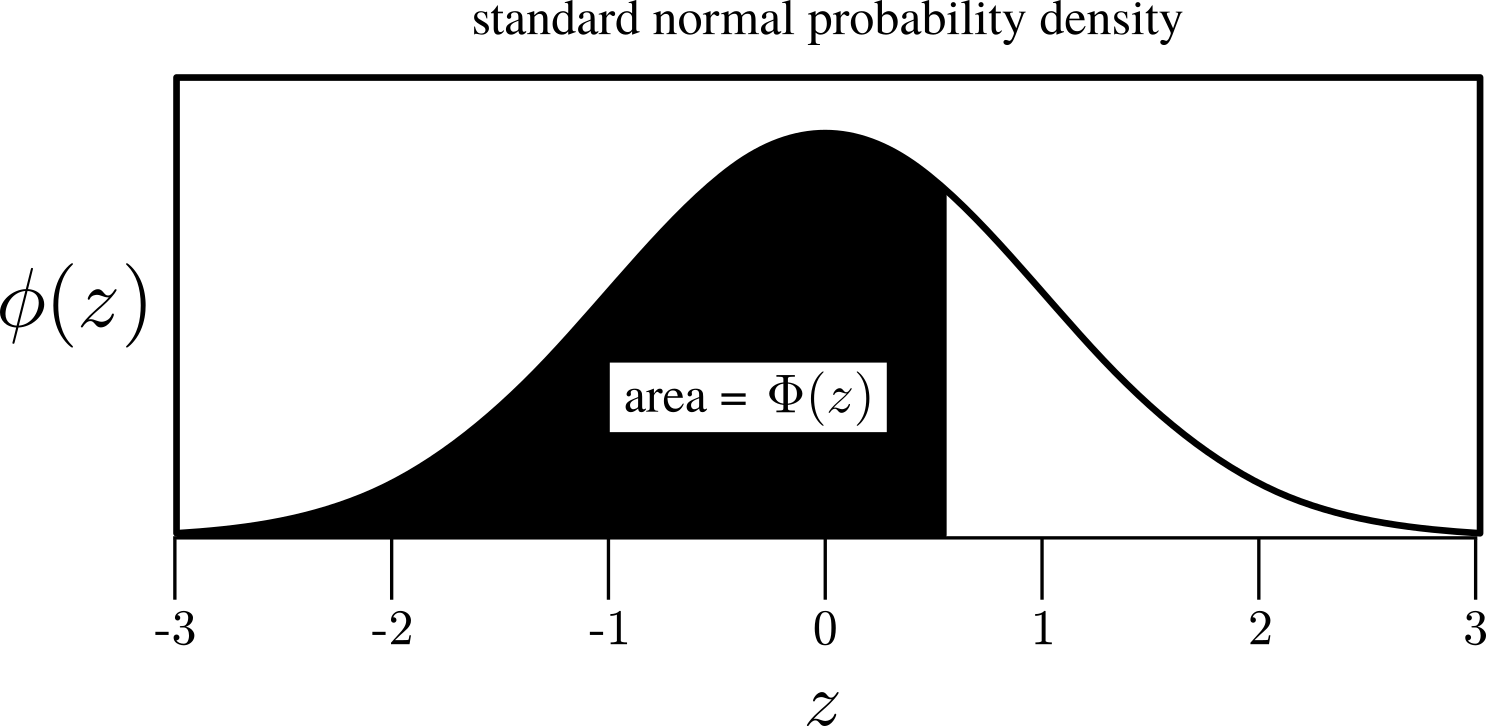
\includegraphics[scale=.7]{area2.png}
\text{ }
\scriptsize 
\begin{multicols}{6}
\begin{tabular}{|c|c|}\hline
$z$ & $\Phi(z)$ \\ \hline
-3.00 & 0.0013\\
-2.98 & 0.0014\\
-2.96 & 0.0015\\
-2.94 & 0.0016\\
-2.92 & 0.0018\\
-2.90 & 0.0019\\
-2.88 & 0.0020\\
-2.86 & 0.0021\\
-2.84 & 0.0023\\
-2.82 & 0.0024\\
-2.80 & 0.0026\\
-2.78 & 0.0027\\
-2.76 & 0.0029\\
-2.74 & 0.0031\\
-2.72 & 0.0033\\
-2.70 & 0.0035\\
-2.68 & 0.0037\\
-2.66 & 0.0039\\
-2.64 & 0.0041\\
-2.62 & 0.0044\\
-2.60 & 0.0047\\
-2.58 & 0.0049\\
-2.56 & 0.0052\\
-2.54 & 0.0055\\
-2.52 & 0.0059\\
-2.50 & 0.0062\\
-2.48 & 0.0066\\
-2.46 & 0.0069\\
-2.44 & 0.0073\\
-2.42 & 0.0078\\
-2.40 & 0.0082\\
-2.38 & 0.0087\\
-2.36 & 0.0091\\
-2.34 & 0.0096\\
-2.32 & 0.0102\\
-2.30 & 0.0107\\
-2.28 & 0.0113\\
-2.26 & 0.0119\\
-2.24 & 0.0125\\
-2.22 & 0.0132\\
-2.20 & 0.0139\\
-2.18 & 0.0146\\
-2.16 & 0.0154\\
-2.14 & 0.0162\\
-2.12 & 0.0170\\
-2.10 & 0.0179\\
-2.08 & 0.0188\\
-2.06 & 0.0197\\
-2.04 & 0.0207\\
-2.02 & 0.0217\\
-2.00 & 0.0228\\
\hline \end{tabular}

\begin{tabular}{|c|c|}\hline
$z$ & $\Phi(z)$ \\ \hline
-2.00 & 0.0228\\
-1.98 & 0.0239\\
-1.96 & 0.0250\\
-1.94 & 0.0262\\
-1.92 & 0.0274\\
-1.90 & 0.0287\\
-1.88 & 0.0301\\
-1.86 & 0.0314\\
-1.84 & 0.0329\\
-1.82 & 0.0344\\
-1.80 & 0.0359\\
-1.78 & 0.0375\\
-1.76 & 0.0392\\
-1.74 & 0.0409\\
-1.72 & 0.0427\\
-1.70 & 0.0446\\
-1.68 & 0.0465\\
-1.66 & 0.0485\\
-1.64 & 0.0505\\
-1.62 & 0.0526\\
-1.60 & 0.0548\\
-1.58 & 0.0571\\
-1.56 & 0.0594\\
-1.54 & 0.0618\\
-1.52 & 0.0643\\
-1.50 & 0.0668\\
-1.48 & 0.0694\\
-1.46 & 0.0721\\
-1.44 & 0.0749\\
-1.42 & 0.0778\\
-1.40 & 0.0808\\
-1.38 & 0.0838\\
-1.36 & 0.0869\\
-1.34 & 0.0901\\
-1.32 & 0.0934\\
-1.30 & 0.0968\\
-1.28 & 0.1003\\
-1.26 & 0.1038\\
-1.24 & 0.1075\\
-1.22 & 0.1112\\
-1.20 & 0.1151\\
-1.18 & 0.1190\\
-1.16 & 0.1230\\
-1.14 & 0.1271\\
-1.12 & 0.1314\\
-1.10 & 0.1357\\
-1.08 & 0.1401\\
-1.06 & 0.1446\\
-1.04 & 0.1492\\
-1.02 & 0.1539\\
-1.00 & 0.1587\\
\hline \end{tabular}

\begin{tabular}{|c|c|}\hline
$z$ & $\Phi(z)$ \\ \hline
-1.00 & 0.1587\\
-0.98 & 0.1635\\
-0.96 & 0.1685\\
-0.94 & 0.1736\\
-0.92 & 0.1788\\
-0.90 & 0.1841\\
-0.88 & 0.1894\\
-0.86 & 0.1949\\
-0.84 & 0.2005\\
-0.82 & 0.2061\\
-0.80 & 0.2119\\
-0.78 & 0.2177\\
-0.76 & 0.2236\\
-0.74 & 0.2296\\
-0.72 & 0.2358\\
-0.70 & 0.2420\\
-0.68 & 0.2483\\
-0.66 & 0.2546\\
-0.64 & 0.2611\\
-0.62 & 0.2676\\
-0.60 & 0.2743\\
-0.58 & 0.2810\\
-0.56 & 0.2877\\
-0.54 & 0.2946\\
-0.52 & 0.3015\\
-0.50 & 0.3085\\
-0.48 & 0.3156\\
-0.46 & 0.3228\\
-0.44 & 0.3300\\
-0.42 & 0.3372\\
-0.40 & 0.3446\\
-0.38 & 0.3520\\
-0.36 & 0.3594\\
-0.34 & 0.3669\\
-0.32 & 0.3745\\
-0.30 & 0.3821\\
-0.28 & 0.3897\\
-0.26 & 0.3974\\
-0.24 & 0.4052\\
-0.22 & 0.4129\\
-0.20 & 0.4207\\
-0.18 & 0.4286\\
-0.16 & 0.4364\\
-0.14 & 0.4443\\
-0.12 & 0.4522\\
-0.10 & 0.4602\\
-0.08 & 0.4681\\
-0.06 & 0.4761\\
-0.04 & 0.4840\\
-0.02 & 0.4920\\
0.00 & 0.5000\\
\hline \end{tabular}

\begin{tabular}{|c|c|}\hline
$z$ & $\Phi(z)$ \\ \hline
0.00 & 0.5000\\
0.02 & 0.5080\\
0.04 & 0.5160\\
0.06 & 0.5239\\
0.08 & 0.5319\\
0.10 & 0.5398\\
0.12 & 0.5478\\
0.14 & 0.5557\\
0.16 & 0.5636\\
0.18 & 0.5714\\
0.20 & 0.5793\\
0.22 & 0.5871\\
0.24 & 0.5948\\
0.26 & 0.6026\\
0.28 & 0.6103\\
0.30 & 0.6179\\
0.32 & 0.6255\\
0.34 & 0.6331\\
0.36 & 0.6406\\
0.38 & 0.6480\\
0.40 & 0.6554\\
0.42 & 0.6628\\
0.44 & 0.6700\\
0.46 & 0.6772\\
0.48 & 0.6844\\
0.50 & 0.6915\\
0.52 & 0.6985\\
0.54 & 0.7054\\
0.56 & 0.7123\\
0.58 & 0.7190\\
0.60 & 0.7257\\
0.62 & 0.7324\\
0.64 & 0.7389\\
0.66 & 0.7454\\
0.68 & 0.7517\\
0.70 & 0.7580\\
0.72 & 0.7642\\
0.74 & 0.7704\\
0.76 & 0.7764\\
0.78 & 0.7823\\
0.80 & 0.7881\\
0.82 & 0.7939\\
0.84 & 0.7995\\
0.86 & 0.8051\\
0.88 & 0.8106\\
0.90 & 0.8159\\
0.92 & 0.8212\\
0.94 & 0.8264\\
0.96 & 0.8315\\
0.98 & 0.8365\\
1.00 & 0.8413\\
\hline \end{tabular}

\begin{tabular}{|c|c|}\hline
$z$ & $\Phi(z)$ \\ \hline
1.00 & 0.8413\\
1.02 & 0.8461\\
1.04 & 0.8508\\
1.06 & 0.8554\\
1.08 & 0.8599\\
1.10 & 0.8643\\
1.12 & 0.8686\\
1.14 & 0.8729\\
1.16 & 0.8770\\
1.18 & 0.8810\\
1.20 & 0.8849\\
1.22 & 0.8888\\
1.24 & 0.8925\\
1.26 & 0.8962\\
1.28 & 0.8997\\
1.30 & 0.9032\\
1.32 & 0.9066\\
1.34 & 0.9099\\
1.36 & 0.9131\\
1.38 & 0.9162\\
1.40 & 0.9192\\
1.42 & 0.9222\\
1.44 & 0.9251\\
1.46 & 0.9279\\
1.48 & 0.9306\\
1.50 & 0.9332\\
1.52 & 0.9357\\
1.54 & 0.9382\\
1.56 & 0.9406\\
1.58 & 0.9429\\
1.60 & 0.9452\\
1.62 & 0.9474\\
1.64 & 0.9495\\
1.66 & 0.9515\\
1.68 & 0.9535\\
1.70 & 0.9554\\
1.72 & 0.9573\\
1.74 & 0.9591\\
1.76 & 0.9608\\
1.78 & 0.9625\\
1.80 & 0.9641\\
1.82 & 0.9656\\
1.84 & 0.9671\\
1.86 & 0.9686\\
1.88 & 0.9699\\
1.90 & 0.9713\\
1.92 & 0.9726\\
1.94 & 0.9738\\
1.96 & 0.9750\\
1.98 & 0.9761\\
2.00 & 0.9772\\
\hline \end{tabular}

\begin{tabular}{|c|c|}\hline
$z$ & $\Phi(z)$ \\ \hline
2.00 & 0.9772\\
2.02 & 0.9783\\
2.04 & 0.9793\\
2.06 & 0.9803\\
2.08 & 0.9812\\
2.10 & 0.9821\\
2.12 & 0.9830\\
2.14 & 0.9838\\
2.16 & 0.9846\\
2.18 & 0.9854\\
2.20 & 0.9861\\
2.22 & 0.9868\\
2.24 & 0.9875\\
2.26 & 0.9881\\
2.28 & 0.9887\\
2.30 & 0.9893\\
2.32 & 0.9898\\
2.34 & 0.9904\\
2.36 & 0.9909\\
2.38 & 0.9913\\
2.40 & 0.9918\\
2.42 & 0.9922\\
2.44 & 0.9927\\
2.46 & 0.9931\\
2.48 & 0.9934\\
2.50 & 0.9938\\
2.52 & 0.9941\\
2.54 & 0.9945\\
2.56 & 0.9948\\
2.58 & 0.9951\\
2.60 & 0.9953\\
2.62 & 0.9956\\
2.64 & 0.9959\\
2.66 & 0.9961\\
2.68 & 0.9963\\
2.70 & 0.9965\\
2.72 & 0.9967\\
2.74 & 0.9969\\
2.76 & 0.9971\\
2.78 & 0.9973\\
2.80 & 0.9974\\
2.82 & 0.9976\\
2.84 & 0.9977\\
2.86 & 0.9979\\
2.88 & 0.9980\\
2.90 & 0.9981\\
2.92 & 0.9982\\
2.94 & 0.9984\\
2.96 & 0.9985\\
2.98 & 0.9986\\
3.00 & 0.9987\\
\hline \end{tabular}


\end{multicols}
\end{center}


\newpage
When given an upper bound $z$, we can use the table to find $\Phi$, which is the probability that $Z$ is below $z$. For example, we might be told that $z=0.42$ and be asked for the probability that $Z$ is less than 0.42.  $$P(Z<0.42) = \Phi(0.42) = 0.6628$$
We can also find the probability that $Z$ is greater than a value, as this is the complementary event.
$$P(Z>0.42) = 1-\Phi(0.42) = 1-0.6628 =  0.3372$$
If you are very slick, you might use the symmetry of the normal curve.
$$P(Z>0.42) = \Phi(-0.42) =  0.3372$$
Also, we can find central areas.
$$P(1 < Z < 2) = \Phi(2)-\Phi(1) = 0.9772-0.8413 = 0.1359$$

\begin{enumerate}
\item Evaluate $\Phi(1.96)$
\vfill
\item Evaluate $P(Z < 1.08)$
\vfill
\item Evaluate $P(Z > 1.08)$
\vfill
\item Evaluate $P(1.08 < Z < 1.96)$
\vfill
\item Evaluate $P(|Z| < 1.96)$, which is the same as $P(-1.96 < Z < 1.96)$
\vfill
\item Evaluate $P(|Z| > 1.96)$, which is the same as $P(Z < -1.96 ~~\text{OR}~~ 1.96<Z)$
\vfill
\end{enumerate}


\newpage
This diagram might be useful. Some of the areas seem to add imperfectly because these numbers are all rounded.\\\\
\begin{center}
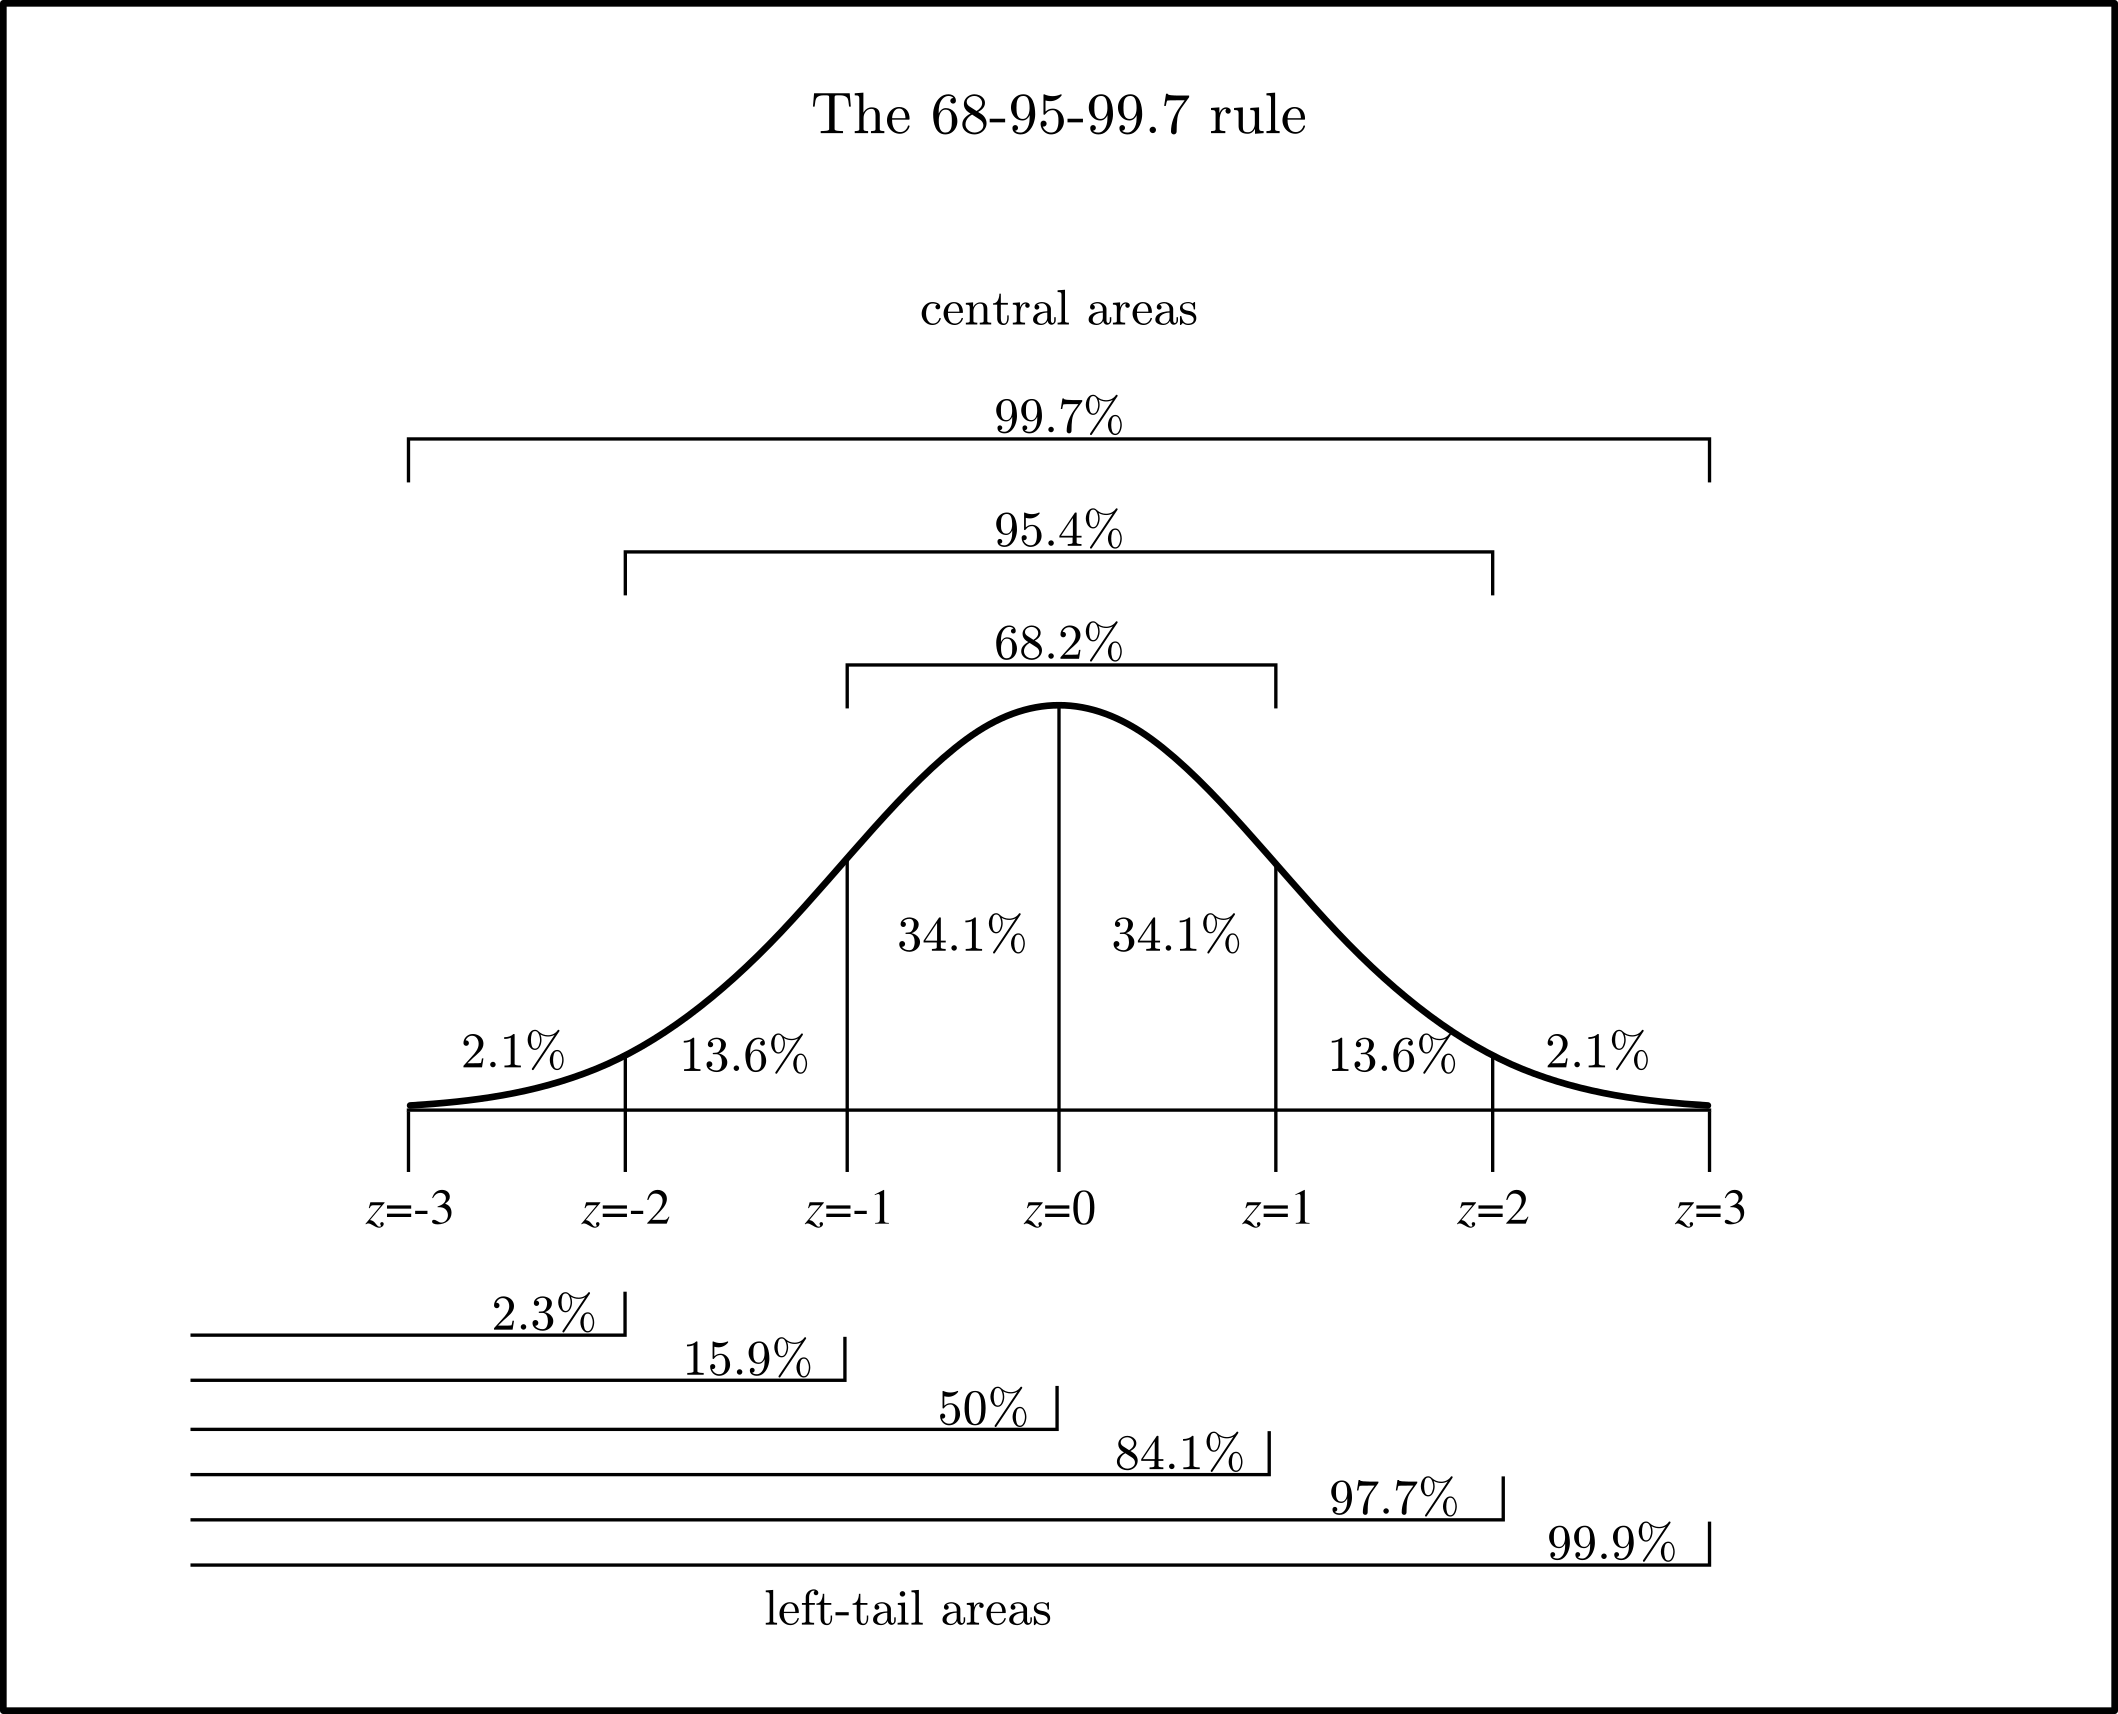
\includegraphics[scale=1]{toomuch2.png}
\end{center}
\url{https://en.wikipedia.org/wiki/68-95-99.7_rule}




\newpage
By using the standard normal table (or the 68-95-99.7 rule), you should be able to determine the following probabilities. For each question, determine the probability (area) of the shaded region or regions. Write the answer using $P(\texttt{condition}) = \texttt{number}$.

\begin{enumerate}[resume,itemsep=50pt]
\begin{multicols}{2}
\item \adjustbox{valign=t}{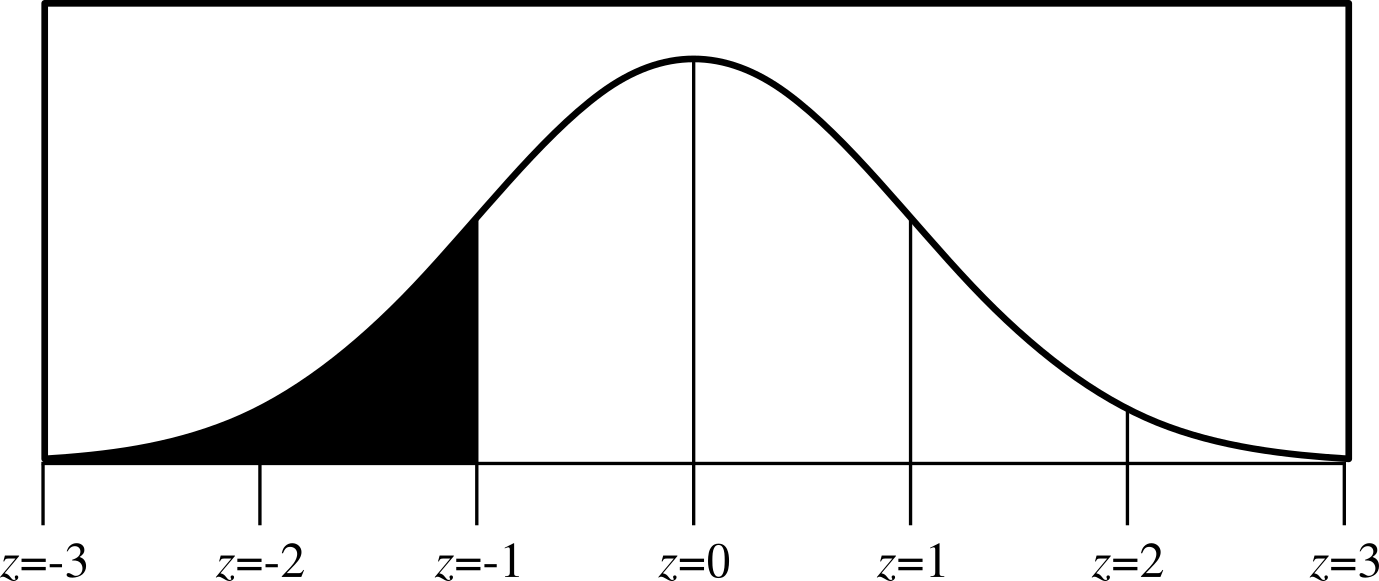
\includegraphics[scale=.5]{n3_n1.png}}
\item \adjustbox{valign=t}{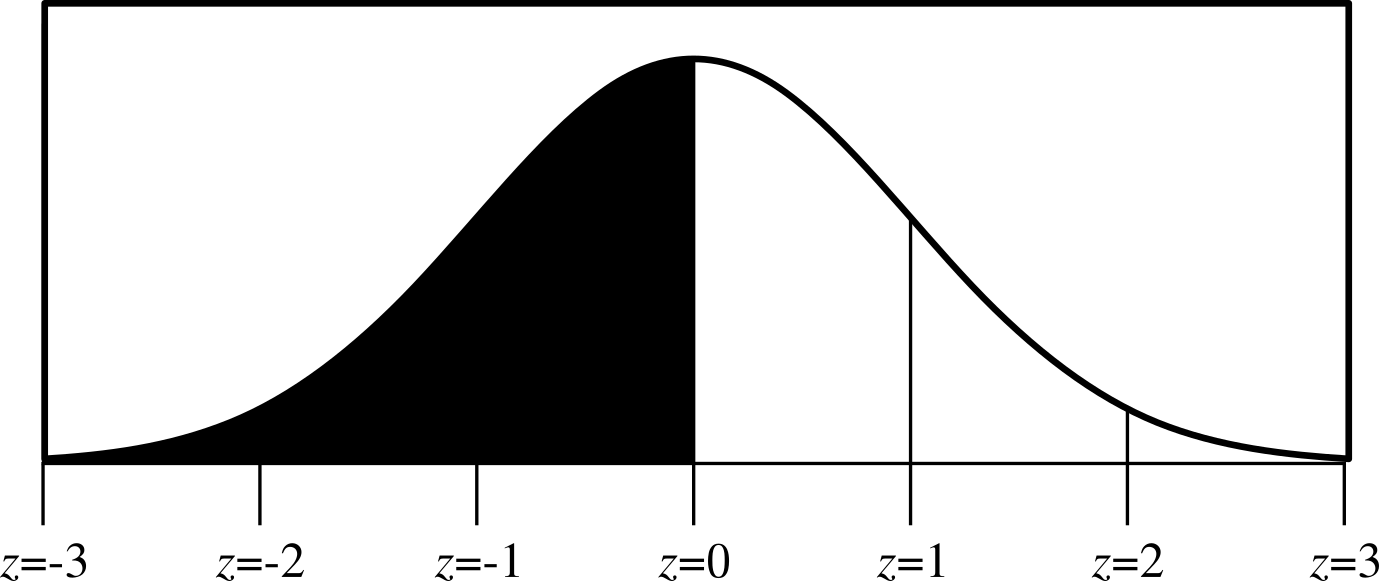
\includegraphics[scale=.5]{n3_0.png}}
\item \adjustbox{valign=t}{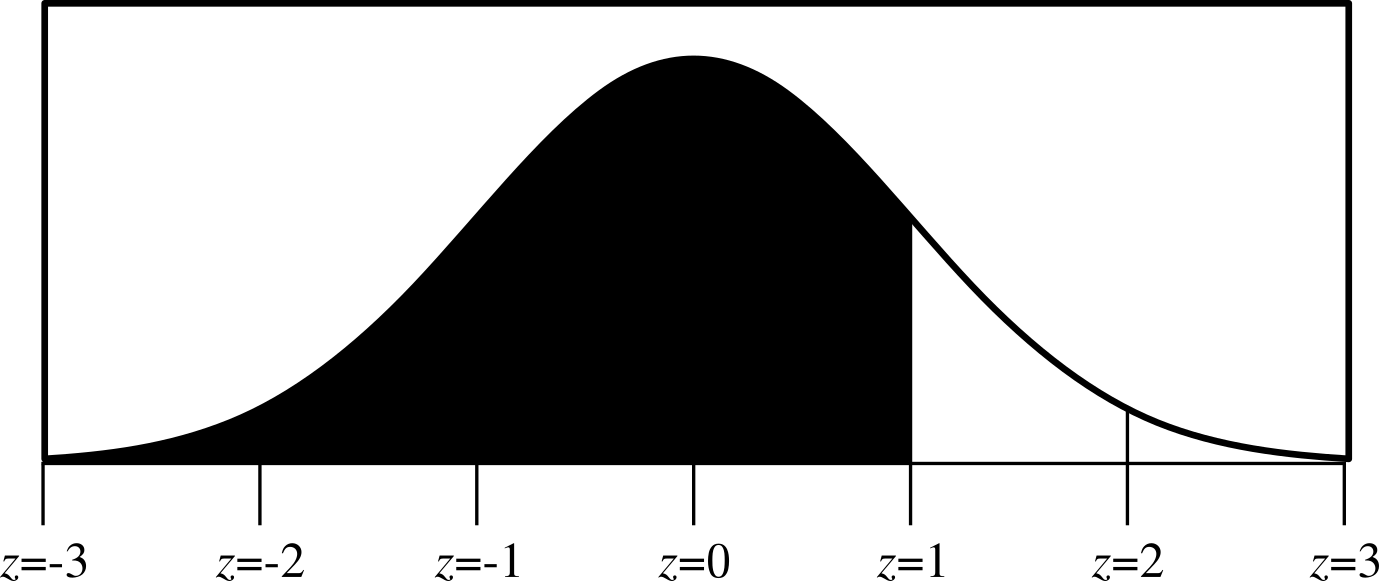
\includegraphics[scale=.5]{n3_1.png}}
\item \adjustbox{valign=t}{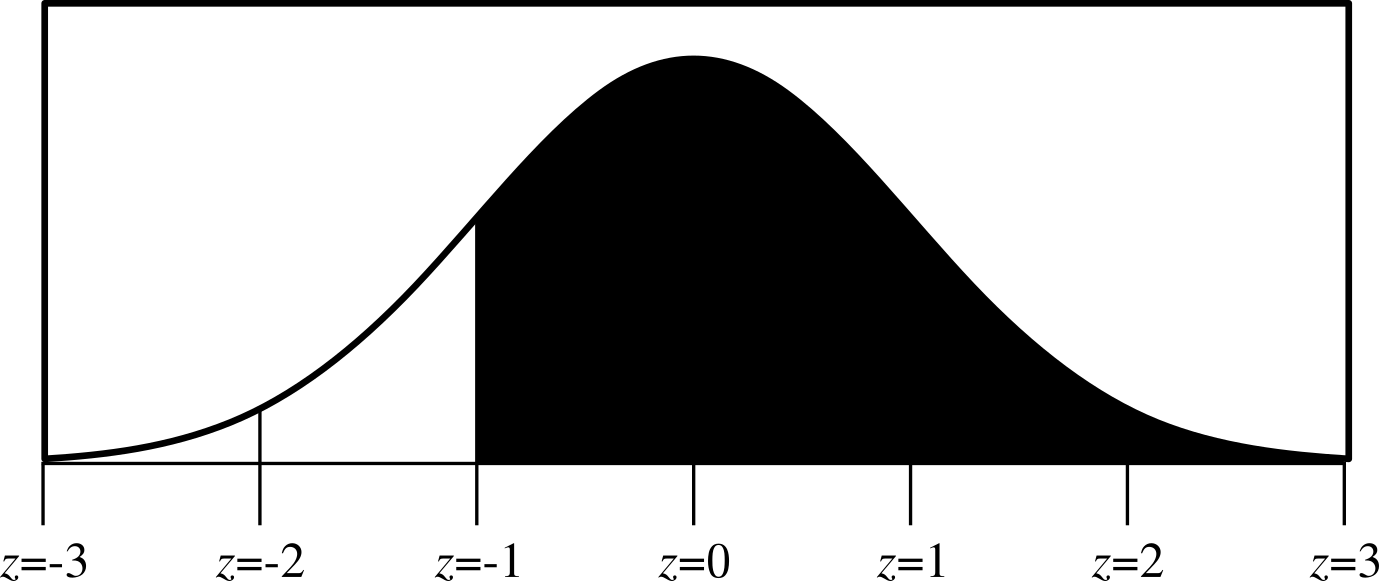
\includegraphics[scale=.5]{n1_3.png}}
\item \adjustbox{valign=t}{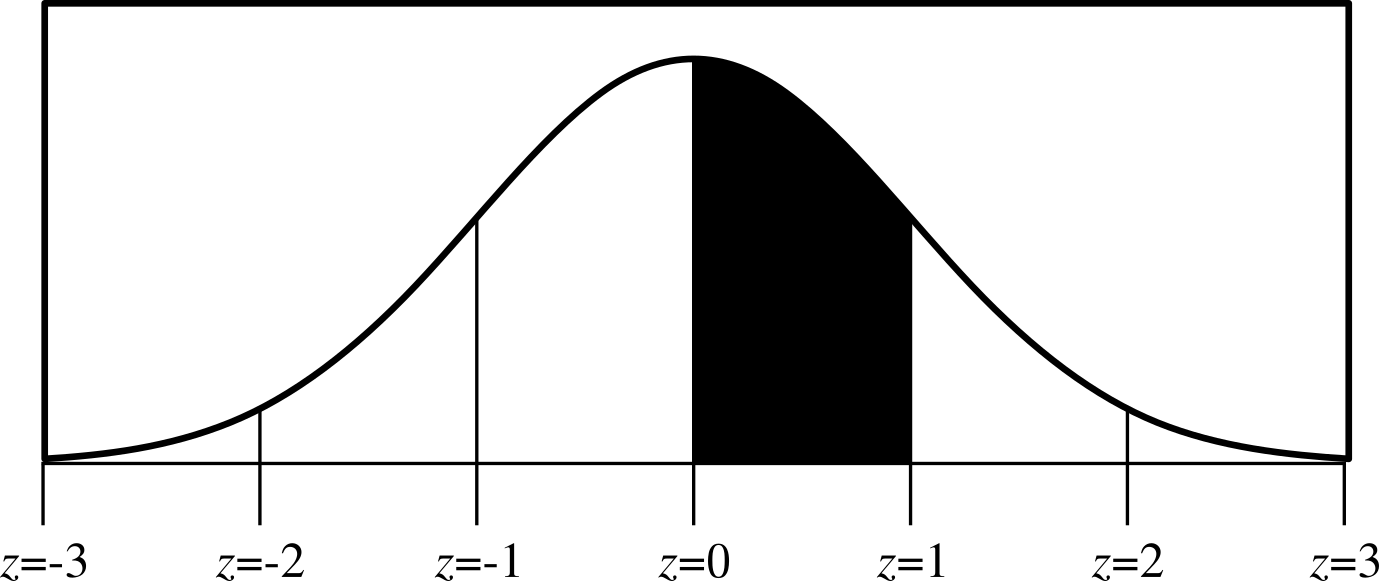
\includegraphics[scale=.5]{0_1.png}}

\columnbreak

\item \adjustbox{valign=t}{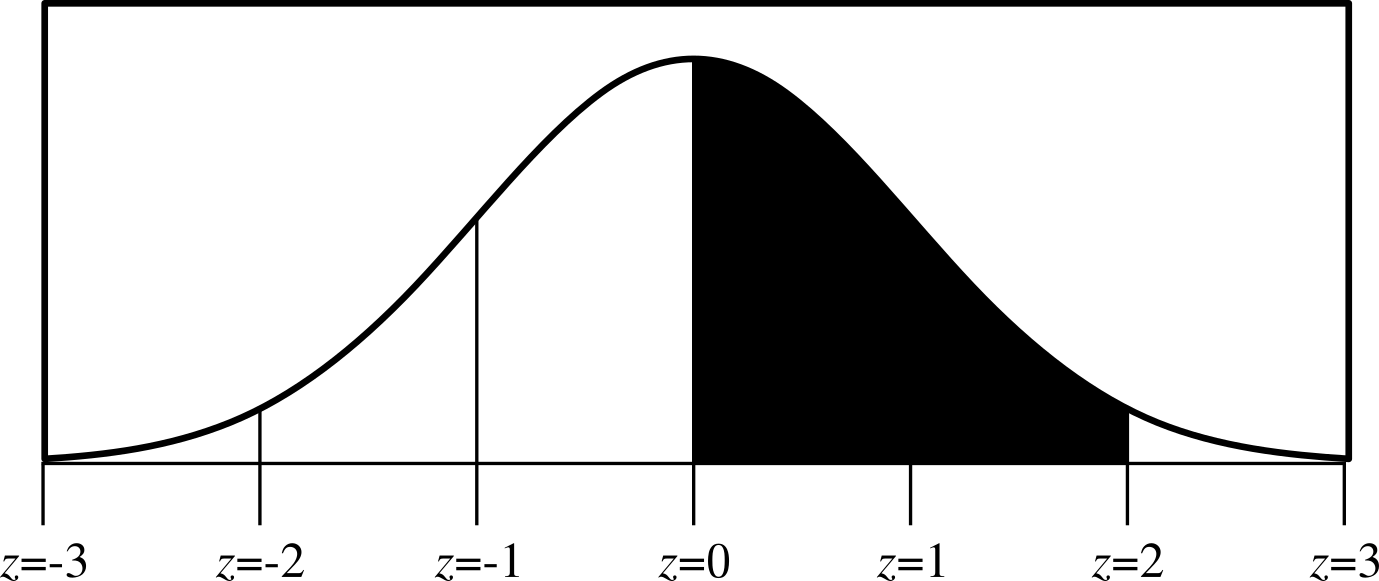
\includegraphics[scale=.5]{0_2.png}}
\item \adjustbox{valign=t}{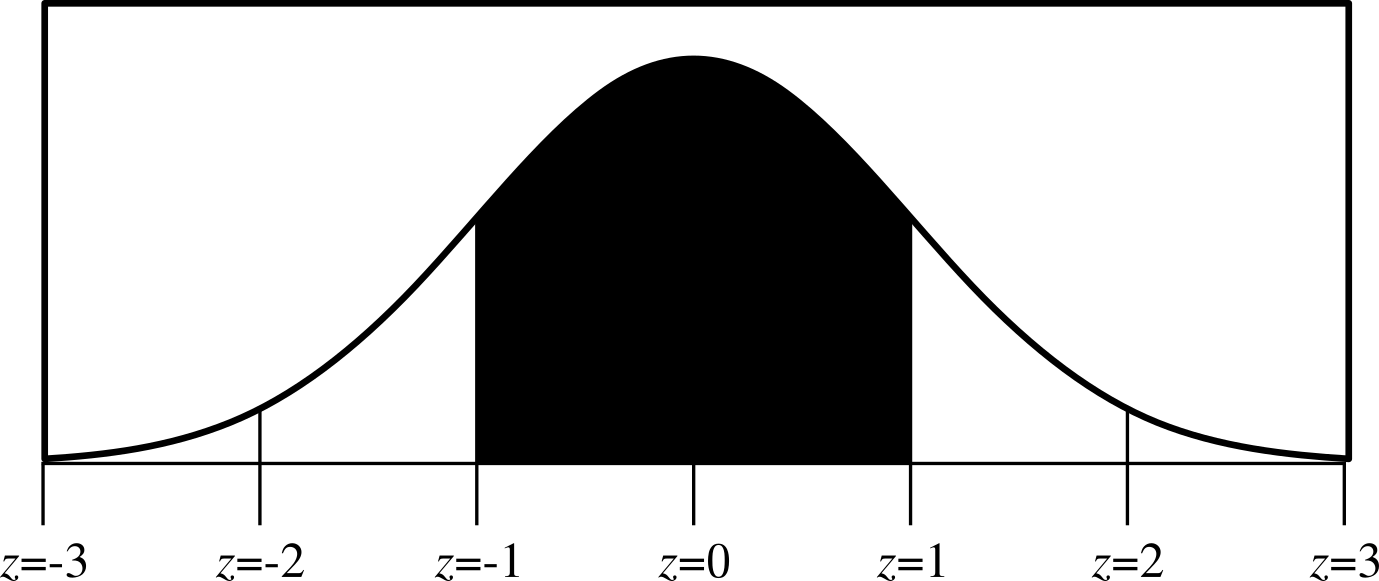
\includegraphics[scale=.5]{n1_1.png}}
\item \adjustbox{valign=t}{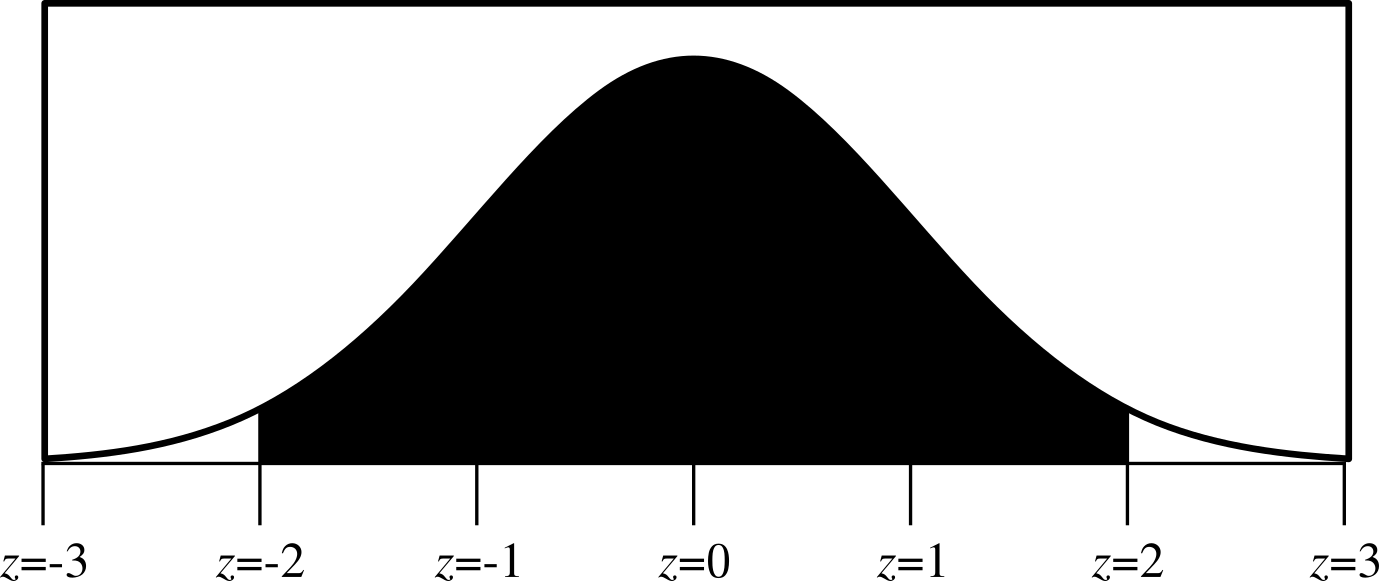
\includegraphics[scale=.5]{n2_2.png}}
\item \adjustbox{valign=t}{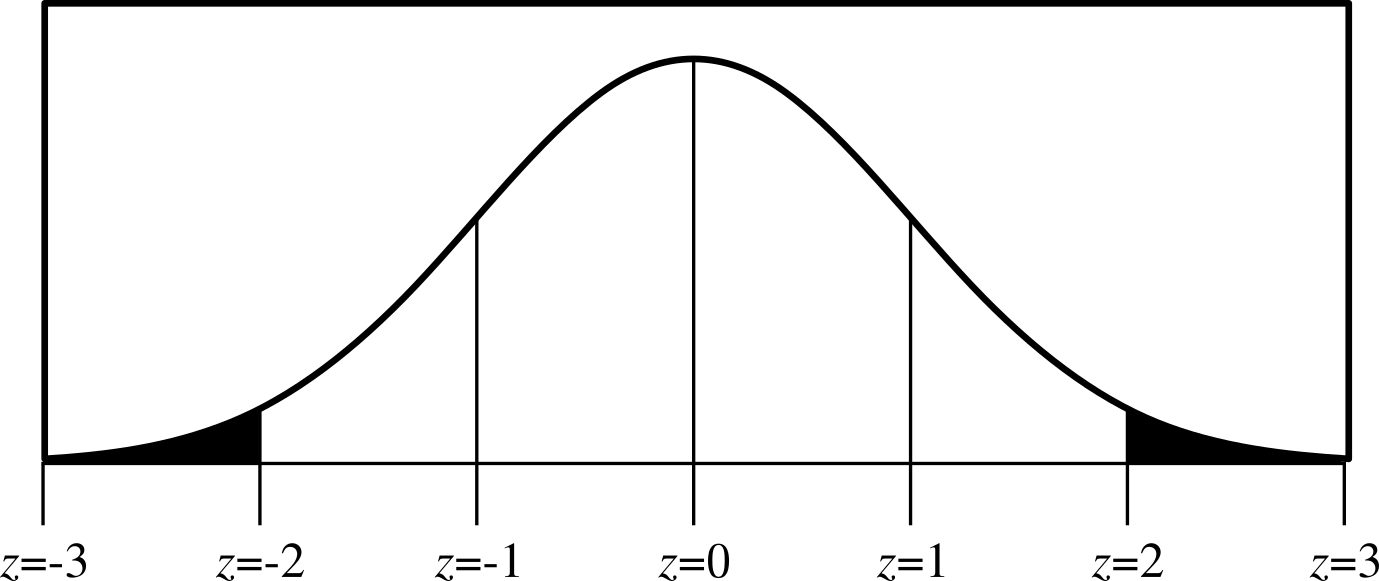
\includegraphics[scale=.5]{n3_n2_and_2_3.png}}
\item \adjustbox{valign=t}{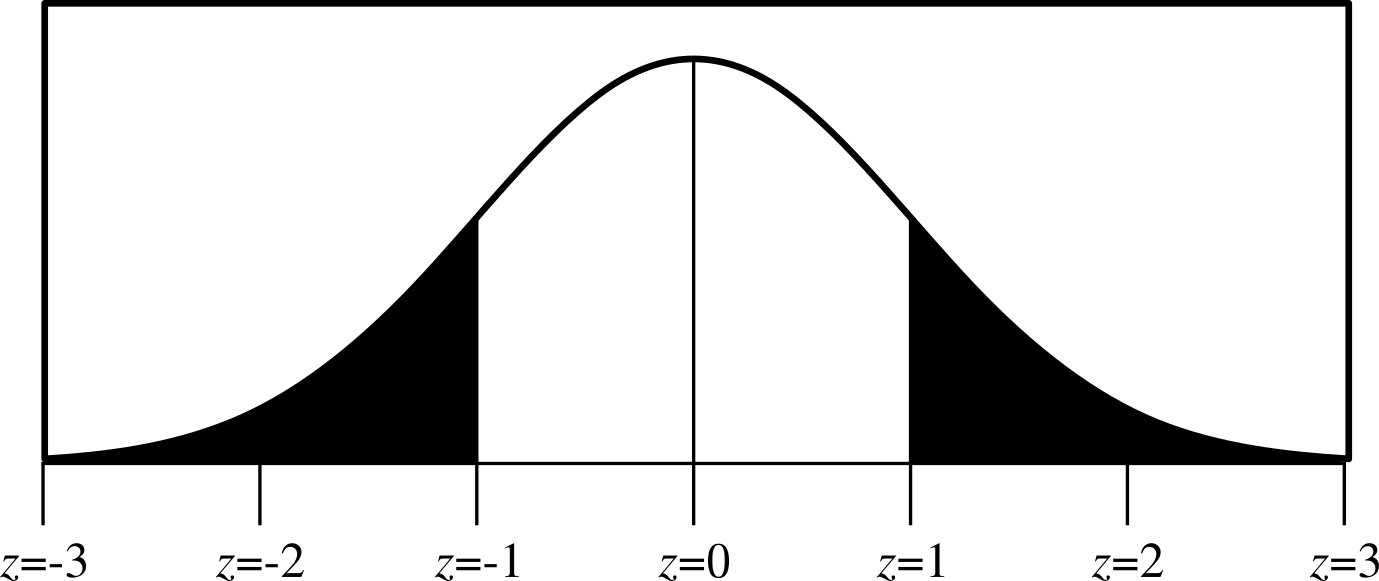
\includegraphics[scale=.5]{n3_n1_and_1_3.png}}

\end{multicols}
\end{enumerate}


\newpage
The cumulative function $\Phi(z)$ is one-to-one, so we can also go backwards! For example, if we wanted to find the value of $z_0$ that satisfies $P(Z<z_0) = 0.86$, we scan the right-columns for $\Phi(z)\approx 0.86$. We find $\Phi(1.08) = 0.8599$.
\begin{center}
\begin{tabular}{|c|c|}\hline
$z$ & $\Phi(z)$ \\ \hline
$\vdots$ & $\vdots$ \\
1.08 & 0.8599 \\
$\vdots$ & $\vdots$ \\ \hline
\end{tabular}
\end{center}
Thus, we estimate $z_0\approx 1.08$. We can also write this as $\Phi^{-1}(0.8599)=1.08$

\begin{enumerate}[resume]
\item Determine $z_0$ such that $\Phi(z_0)=0.0505$. In other words, evaluate $\Phi^{-1}(0.0505)$.
\vfill
\item Determine $z_1$ such that $\Phi(z_1)\approx 0.99$. (Evaluate $\Phi^{-1}(0.99)$.)
\vfill
\item Determine $z_2$ such that $P(Z < z_2) = 55.57\%$
\vfill
\item Determine $z_3$ such that $P(Z > z_3) = 15.87\%$
\vfill
\item Determine $z_4$ such that $P(-z_4 < Z < z_4) = 68.2\%$
\vfill
\item Determine $z_5$ such that $P(|Z| < z_5) = 95\%$
\vfill
\item Determine $z_6$ such that $P(|Z| < z_6) = 90\%$
\vfill
\item Determine $z_7$ such that $P(|Z| > z_7) = 10\%$
\vfill
\end{enumerate}

\newpage

Sometimes it's easier to have an inverse table.
{ \footnotesize
\begin{multicols}{5}
\begin{tabular}{|c|c|}\hline
$\Phi$ & $z$ \\ \hline
0.000 & -inf\\
0.005 & -2.576\\
0.010 & -2.326\\
0.015 & -2.170\\
0.020 & -2.054\\
0.025 & -1.960\\
0.030 & -1.881\\
0.035 & -1.812\\
0.040 & -1.751\\
0.045 & -1.695\\
0.050 & -1.645\\
0.055 & -1.598\\
0.060 & -1.555\\
0.065 & -1.514\\
0.070 & -1.476\\
0.075 & -1.440\\
0.080 & -1.405\\
0.085 & -1.372\\
0.090 & -1.341\\
0.095 & -1.311\\
0.100 & -1.282\\
0.105 & -1.254\\
0.110 & -1.227\\
0.115 & -1.200\\
0.120 & -1.175\\
0.125 & -1.150\\
0.130 & -1.126\\
0.135 & -1.103\\
0.140 & -1.080\\
0.145 & -1.058\\
0.150 & -1.036\\
0.155 & -1.015\\
0.160 & -0.994\\
0.165 & -0.974\\
0.170 & -0.954\\
0.175 & -0.935\\
0.180 & -0.915\\
0.185 & -0.896\\
0.190 & -0.878\\
0.195 & -0.860\\
0.200 & -0.842\\
\hline \end{tabular}

\columnbreak

\begin{tabular}{|c|c|}\hline
$\Phi$ & $z$ \\ \hline
0.200 & -0.842\\
0.205 & -0.824\\
0.210 & -0.806\\
0.215 & -0.789\\
0.220 & -0.772\\
0.225 & -0.755\\
0.230 & -0.739\\
0.235 & -0.722\\
0.240 & -0.706\\
0.245 & -0.690\\
0.250 & -0.674\\
0.255 & -0.659\\
0.260 & -0.643\\
0.265 & -0.628\\
0.270 & -0.613\\
0.275 & -0.598\\
0.280 & -0.583\\
0.285 & -0.568\\
0.290 & -0.553\\
0.295 & -0.539\\
0.300 & -0.524\\
0.305 & -0.510\\
0.310 & -0.496\\
0.315 & -0.482\\
0.320 & -0.468\\
0.325 & -0.454\\
0.330 & -0.440\\
0.335 & -0.426\\
0.340 & -0.412\\
0.345 & -0.399\\
0.350 & -0.385\\
0.355 & -0.372\\
0.360 & -0.358\\
0.365 & -0.345\\
0.370 & -0.332\\
0.375 & -0.319\\
0.380 & -0.305\\
0.385 & -0.292\\
0.390 & -0.279\\
0.395 & -0.266\\
0.400 & -0.253\\
\hline \end{tabular}

\columnbreak

\begin{tabular}{|c|c|}\hline
$\Phi$ & $z$ \\ \hline
0.400 & -0.253\\
0.405 & -0.240\\
0.410 & -0.228\\
0.415 & -0.215\\
0.420 & -0.202\\
0.425 & -0.189\\
0.430 & -0.176\\
0.435 & -0.164\\
0.440 & -0.151\\
0.445 & -0.138\\
0.450 & -0.126\\
0.455 & -0.113\\
0.460 & -0.100\\
0.465 & -0.088\\
0.470 & -0.075\\
0.475 & -0.063\\
0.480 & -0.050\\
0.485 & -0.038\\
0.490 & -0.025\\
0.495 & -0.013\\
0.500 & 0.000\\
0.505 & 0.013\\
0.510 & 0.025\\
0.515 & 0.038\\
0.520 & 0.050\\
0.525 & 0.063\\
0.530 & 0.075\\
0.535 & 0.088\\
0.540 & 0.100\\
0.545 & 0.113\\
0.550 & 0.126\\
0.555 & 0.138\\
0.560 & 0.151\\
0.565 & 0.164\\
0.570 & 0.176\\
0.575 & 0.189\\
0.580 & 0.202\\
0.585 & 0.215\\
0.590 & 0.228\\
0.595 & 0.240\\
0.600 & 0.253\\
\hline \end{tabular}

\columnbreak

\begin{tabular}{|c|c|}\hline
$\Phi$ & $z$ \\ \hline
0.600 & 0.253\\
0.605 & 0.266\\
0.610 & 0.279\\
0.615 & 0.292\\
0.620 & 0.305\\
0.625 & 0.319\\
0.630 & 0.332\\
0.635 & 0.345\\
0.640 & 0.358\\
0.645 & 0.372\\
0.650 & 0.385\\
0.655 & 0.399\\
0.660 & 0.412\\
0.665 & 0.426\\
0.670 & 0.440\\
0.675 & 0.454\\
0.680 & 0.468\\
0.685 & 0.482\\
0.690 & 0.496\\
0.695 & 0.510\\
0.700 & 0.524\\
0.705 & 0.539\\
0.710 & 0.553\\
0.715 & 0.568\\
0.720 & 0.583\\
0.725 & 0.598\\
0.730 & 0.613\\
0.735 & 0.628\\
0.740 & 0.643\\
0.745 & 0.659\\
0.750 & 0.674\\
0.755 & 0.690\\
0.760 & 0.706\\
0.765 & 0.722\\
0.770 & 0.739\\
0.775 & 0.755\\
0.780 & 0.772\\
0.785 & 0.789\\
0.790 & 0.806\\
0.795 & 0.824\\
0.800 & 0.842\\
\hline \end{tabular}

\columnbreak

\begin{tabular}{|c|c|}\hline
$\Phi$ & $z$ \\ \hline
0.800 & 0.842\\
0.805 & 0.860\\
0.810 & 0.878\\
0.815 & 0.896\\
0.820 & 0.915\\
0.825 & 0.935\\
0.830 & 0.954\\
0.835 & 0.974\\
0.840 & 0.994\\
0.845 & 1.015\\
0.850 & 1.036\\
0.855 & 1.058\\
0.860 & 1.080\\
0.865 & 1.103\\
0.870 & 1.126\\
0.875 & 1.150\\
0.880 & 1.175\\
0.885 & 1.200\\
0.890 & 1.227\\
0.895 & 1.254\\
0.900 & 1.282\\
0.905 & 1.311\\
0.910 & 1.341\\
0.915 & 1.372\\
0.920 & 1.405\\
0.925 & 1.440\\
0.930 & 1.476\\
0.935 & 1.514\\
0.940 & 1.555\\
0.945 & 1.598\\
0.950 & 1.645\\
0.955 & 1.695\\
0.960 & 1.751\\
0.965 & 1.812\\
0.970 & 1.881\\
0.975 & 1.960\\
0.980 & 2.054\\
0.985 & 2.170\\
0.990 & 2.326\\
0.995 & 2.576\\
1.000 & inf\\
\hline \end{tabular}

\columnbreak


\end{multicols}
}


\newpage
We need to introduce three new variables: $\alpha$, $\gamma$, and $z^*$. These are pronounced ``alpha'', ``gamma'', and ``z star''.

\begin{center}
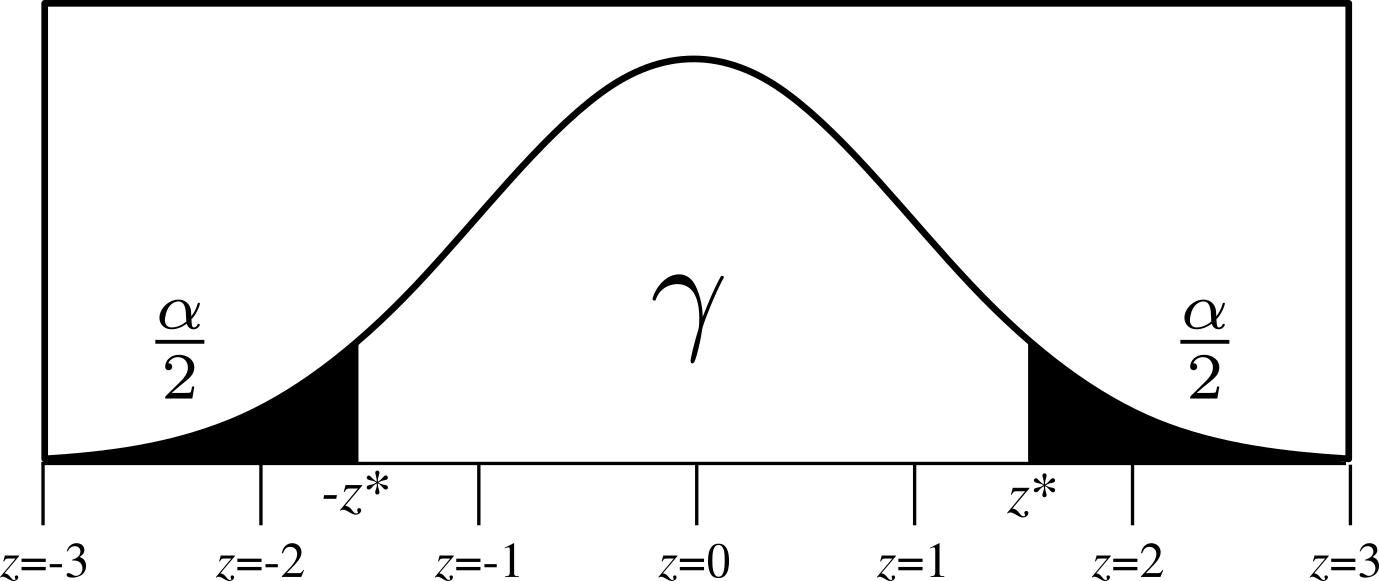
\includegraphics[scale=1]{alphagamma.png}
\end{center}

In this situation, we have a central area which is symmetric about $z=0$. In other words, it stretches equally far to the left as to the right. In fact, it stretches from $-z^*$ to $z^*$. The area in the middle is $\gamma$. The combined area of the tails is $\alpha$.
$$\gamma = P(-z^* < Z < z^*)$$
$$\gamma = P(|Z| < z^*)$$
$$\gamma = \Phi(z^*)-\Phi(-z^*) $$
$$\gamma = 2\Phi(z^*)-1 $$

$$\alpha = 1-\gamma $$
$$\alpha = P(|Z| > z^*) $$
$$\alpha = 2(1-\Phi(z^*)) $$
In the context of confidence intervals, $\gamma$ is called the confidence level and $z^*$ is called the critical $z$.

{ \footnotesize
\begin{multicols}{2}
\begin{tabular}{|c|c|c|c|}\hline
$\gamma$ & $\alpha$ & $\Phi$ & $z$ \\ \hline
0.50 & 0.50 & 0.750 & 0.674\\
0.51 & 0.49 & 0.755 & 0.690\\
0.52 & 0.48 & 0.760 & 0.706\\
0.53 & 0.47 & 0.765 & 0.722\\
0.54 & 0.46 & 0.770 & 0.739\\
0.55 & 0.45 & 0.775 & 0.755\\
0.56 & 0.44 & 0.780 & 0.772\\
0.57 & 0.43 & 0.785 & 0.789\\
0.58 & 0.42 & 0.790 & 0.806\\
0.59 & 0.41 & 0.795 & 0.824\\
0.60 & 0.40 & 0.800 & 0.842\\
0.61 & 0.39 & 0.805 & 0.860\\
0.62 & 0.38 & 0.810 & 0.878\\
0.63 & 0.37 & 0.815 & 0.896\\
0.64 & 0.36 & 0.820 & 0.915\\
0.65 & 0.35 & 0.825 & 0.935\\
0.66 & 0.34 & 0.830 & 0.954\\
0.67 & 0.33 & 0.835 & 0.974\\
0.68 & 0.32 & 0.840 & 0.994\\
0.69 & 0.31 & 0.845 & 1.015\\
0.70 & 0.30 & 0.850 & 1.036\\
0.71 & 0.29 & 0.855 & 1.058\\
0.72 & 0.28 & 0.860 & 1.080\\
0.73 & 0.27 & 0.865 & 1.103\\
0.74 & 0.26 & 0.870 & 1.126\\
0.75 & 0.25 & 0.875 & 1.150\\
\hline \end{tabular}

\columnbreak

\begin{tabular}{|c|c|c|c|}\hline
$\gamma$ & $\alpha$ & $\Phi$ & $z$ \\ \hline
0.75 & 0.25 & 0.875 & 1.150\\
0.76 & 0.24 & 0.880 & 1.175\\
0.77 & 0.23 & 0.885 & 1.200\\
0.78 & 0.22 & 0.890 & 1.227\\
0.79 & 0.21 & 0.895 & 1.254\\
0.80 & 0.20 & 0.900 & 1.282\\
0.81 & 0.19 & 0.905 & 1.311\\
0.82 & 0.18 & 0.910 & 1.341\\
0.83 & 0.17 & 0.915 & 1.372\\
0.84 & 0.16 & 0.920 & 1.405\\
0.85 & 0.15 & 0.925 & 1.440\\
0.86 & 0.14 & 0.930 & 1.476\\
0.87 & 0.13 & 0.935 & 1.514\\
0.88 & 0.12 & 0.940 & 1.555\\
0.89 & 0.11 & 0.945 & 1.598\\
0.90 & 0.10 & 0.950 & 1.645\\
0.91 & 0.09 & 0.955 & 1.695\\
0.92 & 0.08 & 0.960 & 1.751\\
0.93 & 0.07 & 0.965 & 1.812\\
0.94 & 0.06 & 0.970 & 1.881\\
0.95 & 0.05 & 0.975 & 1.960\\
0.96 & 0.04 & 0.980 & 2.054\\
0.97 & 0.03 & 0.985 & 2.170\\
0.98 & 0.02 & 0.990 & 2.326\\
0.99 & 0.01 & 0.995 & 2.576\\
1.00 & 0.00 & 1.000 & inf\\
\hline \end{tabular}

\columnbreak


\end{multicols}
}


\newpage
If the random variable $\bar{X}$ is the mean of a sample of size $n$ from {\bf any} distribution with mean $\mu$ and standard deviation $\sigma$, then we know $\bar{X}$ is approximately normal with mean $\mu$ and standard deviation $\frac{\sigma}{\sqrt{n}}$. We say the {\bf sampling distribution} of the {\bf sample mean} has a standard error of $\frac{\sigma}{\sqrt{n}}$.

Now, imagine you sampled 100 random beans from a huge bag, and those 100 beans had a mean mass of 13.71 grams. Also, somehow, you know the population's standard deviation is 0.83 grams. You know the whole bag could have a mean mass that is {\bf not} 13.71 grams; in fact, you guess it is quite unlikely that the sample has the exact same mean mass as the population. However, you also doubt the population's mean is 10 grams or 20 grams. From this idea, we develop the {\bf confidence interval}. We, informally, want an interval with a 95\% chance of including the true population's mean.

\newcommand{\ME}{\mathtt{ME}}
\newcommand{\SE}{\sigma_{\bar{x}}}


\begin{enumerate}[resume]
\item Calculate $\sigma_{\bar{x}}$, the standard error of the mean, if $\sigma = 0.83$ and $n=100$.
\vfill
\item Determine $z^*$ such that $P(|Z| < z^*) = 95\%$. \\This is equivalent to finding $z^*$ that satisfies $\Phi(z^*)=0.975$.\\
This is equivalent to evaluating $\Phi^{-1}(0.975)$.
\vfill
\item Calculate the {\bf margin of error} by multiplying $\SE$ and $z^*$. (I could not find any text using a variable other than $\ME$ to represent margin of error.)
$$\ME = (z^*)(\SE) =$$
\vfill
\item Calculate the lower bound of the interval.\\
$\texttt{lower bound of 95\% confidency interval} = 13.71-\ME = $
\vfill
\item Calculate the upper bound of the interval.\\
$\texttt{upper bound of 95\% confidency interval} = 13.71+\ME = $
\vfill
\end{enumerate}

\newpage
\subsection*{Calculating a confidence interval of mean with known population standard deviation}
You are given the following:

\begin{tabular}{|c|c|c|}\hline
name & variable & value from previous example \\ \hline
sample mean & $\bar{x}$ & 13.71 \\
sample size & $n$ & 100 \\
population standard deviation & $\sigma$ & 0.83 \\
confidence level & $\gamma$ & 0.95 \\ \hline
\end{tabular}\\

\vspace{20pt}

\begin{itemize}
\item Determine the standard error.
$$\SE = \frac{\sigma}{\sqrt{n}} $$
\item Calculate $\alpha$, the two-tail complement of $\gamma$.
$$\alpha = 1-\gamma $$

\item Determine $z^*$ such that $\Phi(z^*) = 1-\cfrac{\alpha}{2}$.
$$z^* = \Phi^{-1}\left(1-\cfrac{\alpha}{2}\right) $$
For typical values of $\gamma$, the following table will help.
\begin{center}
\begin{tabular}{|c|c|c|c|c|c|}\hline
$\gamma$ & $\alpha$ & $1-\frac{\alpha}{2}$ & $\Phi(z^*)$ & $\Phi^{-1}(\Phi(z^*))$ & $z^*$ \\ \hline
0.9 & 0.1 & 0.95 & 0.95 & 1.645 & 1.645 \\
0.95 & 0.05 & 0.975 & 0.975 & 1.96 & 1.96 \\
0.98 & 0.02 & 0.99 & 0.99 & 2.326 & 2.326\\
0.99 & 0.01 & 0.995 & 0.995 & 2.576 & 2.576\\ \hline
\end{tabular}
\end{center}

\item Calculate the margin of error.
$$\ME = (z^*)(\SE) $$

\item Calculate the lower bound.
$$\texttt{lower bound of confidence interval} = \bar{x}-\ME $$
\item Calculate the upper bound.
$$\texttt{upper bound of confidence interval} = \bar{x}+\ME $$
\item Interpret.\\
``With a confidence level of \fbox{\phantom{H} $\gamma$ \phantom{H}}, the true mean is between \fbox{\phantom{H} LB \phantom{H}} and \fbox{\phantom{H} UB \phantom{H}}.''
\end{itemize}
\url{https://en.wikipedia.org/wiki/Confidence_interval#Basic_steps}
\newpage
\begin{enumerate}[resume]
\item A sample of size 36 is taken from a distribution with a standard deviation of 20. The mean of the sample is 150. Calculate a 95\% confidence interval of the population's mean.
\vfill
\item A sample of size 49 is taken from a distribution with a standard deviation of 14. The mean of the sample is 88. Calculate a 80\% confidence interval of the population's mean.
\vfill

\end{enumerate}

\newpage
\subsection*{Calculating a confidence interval of mean using sample's standard deviation}
In science, we are unlikely to know the population's true standard deviation. When we do not know the population's standard deviation, we make a subtle change to the calculations: we use Student's $t$ distribution.

You are given the following:

\begin{tabular}{|c|c|}\hline
name & variable  \\ \hline
sample mean & $\bar{x}$  \\
sample size & $n$ \\
sample standard deviation & $s$ \\
confidence level & $\gamma$ \\ \hline
\end{tabular}\\
\begin{itemize}
\item Estimate the standard error.
$$s_{\bar{x}} = \frac{s}{\sqrt{n}} $$
\item Calculate $\alpha$, the two-tail complement of $\gamma$.
$$\alpha = 1-\gamma $$
\item Calculate the degrees of freedom, $df$.
$$df = n-1$$
\item Determine $t^*$ from $\alpha$ and $df$. You look up $t^*$ in the table. These are only presented as an inverse table.


\item Calculate the margin of error.
$$\ME = (t^*)(s_{\bar{x}}) $$

\item Calculate the lower bound.
$$\texttt{lower bound of confidence interval} = \bar{x}-\ME $$
\item Calculate the upper bound.
$$\texttt{upper bound of confidence interval} = \bar{x}+\ME $$
\item Interpret.\\
``With a confidence level of \fbox{\phantom{H} $\gamma$ \phantom{H}}, the true mean is between \fbox{\phantom{H} LB \phantom{H}} and \fbox{\phantom{H} UB \phantom{H}}.''
\end{itemize}
\url{https://en.wikipedia.org/wiki/Confidence_interval#Basic_steps}
\newpage

\section{Student's $t$ distribution (two-tailed)}

\begin{center}
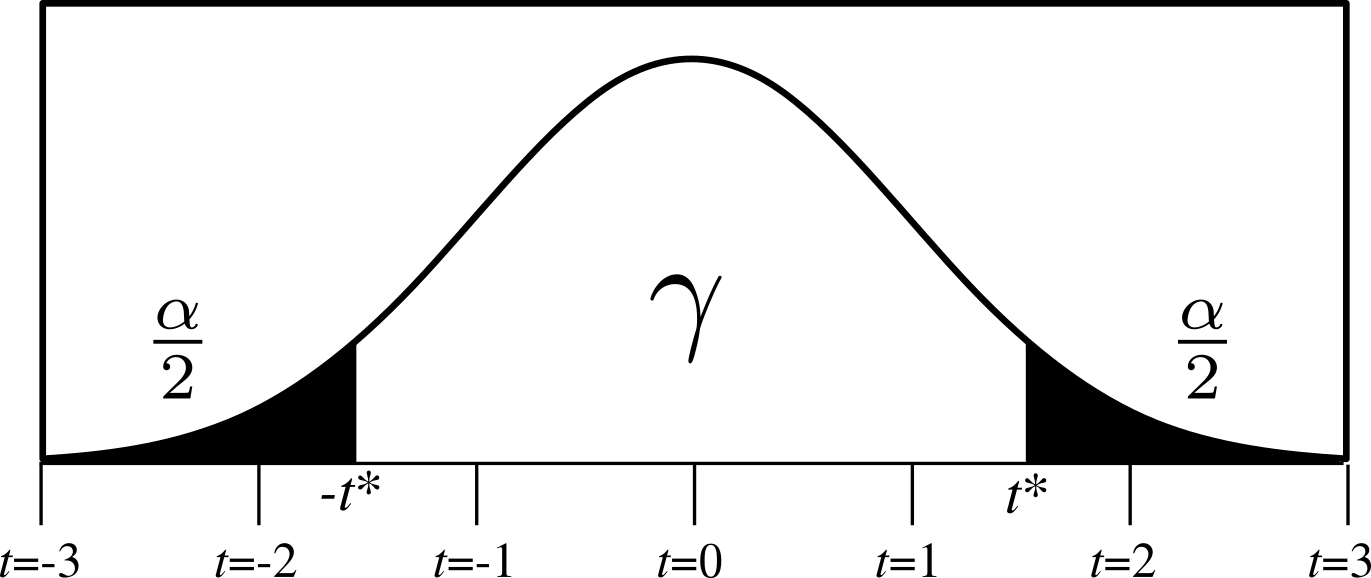
\includegraphics[scale=0.7]{tcurve.png}
\end{center}

The $t$ distribution depends on the degrees of freedom, $$df=n-1$$ Thus, it is customary to pick a few common values of $\alpha$, and display an inverse table with various degrees of freedom.
\vspace{20pt}

{ \footnotesize
\begin{multicols}{5}
\begin{tabular}{|c|c|}\hline
 \multicolumn{2}{|c|}{$\alpha$ = 0.20}\\
$df$ & $t$ \\ \hline
1 & 3.08\\
2 & 1.89\\
3 & 1.64\\
4 & 1.53\\
5 & 1.48\\
6 & 1.44\\
7 & 1.41\\
8 & 1.40\\
9 & 1.38\\
10 & 1.37\\
11 & 1.36\\
12 & 1.36\\
13 & 1.35\\
14 & 1.35\\
15 & 1.34\\
16 & 1.34\\
17 & 1.33\\
18 & 1.33\\
19 & 1.33\\
20 & 1.33\\
21 & 1.32\\
22 & 1.32\\
23 & 1.32\\
24 & 1.32\\
25 & 1.32\\
26 & 1.31\\
27 & 1.31\\
28 & 1.31\\
29 & 1.31\\
30 & 1.31\\
35 & 1.31\\
40 & 1.30\\
50 & 1.30\\
$\infty$ & 1.28\\
\hline \end{tabular}

\begin{tabular}{|c|c|}\hline
 \multicolumn{2}{|c|}{$\alpha$ = 0.10}\\
$df$ & $t$ \\ \hline
1 & 6.31\\
2 & 2.92\\
3 & 2.35\\
4 & 2.13\\
5 & 2.02\\
6 & 1.94\\
7 & 1.89\\
8 & 1.86\\
9 & 1.83\\
10 & 1.81\\
11 & 1.80\\
12 & 1.78\\
13 & 1.77\\
14 & 1.76\\
15 & 1.75\\
16 & 1.75\\
17 & 1.74\\
18 & 1.73\\
19 & 1.73\\
20 & 1.72\\
21 & 1.72\\
22 & 1.72\\
23 & 1.71\\
24 & 1.71\\
25 & 1.71\\
26 & 1.71\\
27 & 1.70\\
28 & 1.70\\
29 & 1.70\\
30 & 1.70\\
35 & 1.69\\
40 & 1.68\\
50 & 1.68\\
$\infty$ & 1.65\\
\hline \end{tabular}

\begin{tabular}{|c|c|}\hline
 \multicolumn{2}{|c|}{$\alpha$ = 0.05}\\
$df$ & $t$ \\ \hline
1 & 12.71\\
2 & 4.30\\
3 & 3.18\\
4 & 2.78\\
5 & 2.57\\
6 & 2.45\\
7 & 2.36\\
8 & 2.31\\
9 & 2.26\\
10 & 2.23\\
11 & 2.20\\
12 & 2.18\\
13 & 2.16\\
14 & 2.14\\
15 & 2.13\\
16 & 2.12\\
17 & 2.11\\
18 & 2.10\\
19 & 2.09\\
20 & 2.09\\
21 & 2.08\\
22 & 2.07\\
23 & 2.07\\
24 & 2.06\\
25 & 2.06\\
26 & 2.06\\
27 & 2.05\\
28 & 2.05\\
29 & 2.05\\
30 & 2.04\\
35 & 2.03\\
40 & 2.02\\
50 & 2.01\\
$\infty$ & 1.96\\
\hline \end{tabular}

\begin{tabular}{|c|c|}\hline
 \multicolumn{2}{|c|}{$\alpha$ = 0.02}\\
$df$ & $t$ \\ \hline
1 & 31.82\\
2 & 6.96\\
3 & 4.54\\
4 & 3.75\\
5 & 3.36\\
6 & 3.14\\
7 & 3.00\\
8 & 2.90\\
9 & 2.82\\
10 & 2.76\\
11 & 2.72\\
12 & 2.68\\
13 & 2.65\\
14 & 2.62\\
15 & 2.60\\
16 & 2.58\\
17 & 2.57\\
18 & 2.55\\
19 & 2.54\\
20 & 2.53\\
21 & 2.52\\
22 & 2.51\\
23 & 2.50\\
24 & 2.49\\
25 & 2.49\\
26 & 2.48\\
27 & 2.47\\
28 & 2.47\\
29 & 2.46\\
30 & 2.46\\
35 & 2.44\\
40 & 2.42\\
50 & 2.40\\
$\infty$ & 2.33\\
\hline \end{tabular}

\begin{tabular}{|c|c|}\hline
 \multicolumn{2}{|c|}{$\alpha$ = 0.01}\\
$df$ & $t$ \\ \hline
1 & 63.66\\
2 & 9.92\\
3 & 5.84\\
4 & 4.60\\
5 & 4.03\\
6 & 3.71\\
7 & 3.50\\
8 & 3.36\\
9 & 3.25\\
10 & 3.17\\
11 & 3.11\\
12 & 3.05\\
13 & 3.01\\
14 & 2.98\\
15 & 2.95\\
16 & 2.92\\
17 & 2.90\\
18 & 2.88\\
19 & 2.86\\
20 & 2.85\\
21 & 2.83\\
22 & 2.82\\
23 & 2.81\\
24 & 2.80\\
25 & 2.79\\
26 & 2.78\\
27 & 2.77\\
28 & 2.76\\
29 & 2.76\\
30 & 2.75\\
35 & 2.72\\
40 & 2.70\\
50 & 2.68\\
$\infty$ & 2.58\\
\hline \end{tabular}


\end{multicols}
}


\newpage
\begin{enumerate}[resume]
\item A sample of size 36 is measured. The mean value is 100 and the sample standard deviation is 24. Calculate a 95\% confidence interval.
\begin{enumerate}
\item Identify the sample mean. ~~ $\bar{x}=$
\item Identify the sample size. ~~$n=$
\item Identify the sample standard deviation. ~~$s=$
\item Identify the confidence level. ~~$\gamma=$
\item Estimate $s_{\bar{x}}$, the standard error. Remember, $s_{\bar{x}}=\frac{s}{\sqrt{n}}$.
\vspace{30pt}
\\$$s_{\bar{x}} = $$
\vspace{10pt}
\item Calculate $\alpha$. Remember, $\alpha = 1-\gamma$.
\vspace{30pt}
\\$$\alpha = $$
\vspace{10pt}
\item Calculate $df$, the degrees of freedom. Remember, $df = n-1$.
\vspace{30pt}
\\$$df = $$
\vspace{10pt}
\item Determine $t^*$ from the table. ~~ $t^*=$
\item Calculate $\ME$, the margin of error. Remember, $\ME = (t^*)(s_{\bar{x}})$.
\vspace{30pt}
\\$$\ME = $$
\vspace{10pt}
\item Calculate the lower bound. Remember, $\texttt{lower bound of confidence interval} = \bar{x}-\ME $.
\vspace{30pt}
\item Calculate the upper bound. Remember, $\texttt{upper bound of confidence interval} = \bar{x}+\ME $.
\vspace{30pt}
\end{enumerate}
\end{enumerate}

\newpage
\begin{enumerate}[resume]
\item A sample of size 31 is measured. The mean value is 40 and the sample standard deviation is 5. Calculate a 95\% confidence interval.
\end{enumerate}

\newpage
\subsection*{Calculating a confidence interval of proportion using normal approximation}
Lastly, we also find confidence intervals of a special mean, the proportion. When we measure failures and successes, and label those with 0s and 1s, then the mean of those 0s and 1s is called a proportion. In this case, the population's proportion $p$ is unknown, but we can calculate our best guess, $\hat{p}$. In this case, the standard deviation can be calculated from $p$ or estimated from $\hat{p}$.
\\
\\
You are given the following:

\begin{tabular}{|c|c|}\hline
name & variable  \\ \hline
number of trials & $n$  \\
number of successes & $n_s$ \\
confidence level & $\gamma$ \\ \hline
\end{tabular}\\
\begin{itemize}
\item Calculate $\hat{p}$, the estimate of the population's proportion.
$$\hat{p} = \frac{n_s}{n} $$
\item Estimate the standard error.
$$s_{\hat{p}} = \frac{\sqrt{\hat{p}(1-\hat{p})}}{\sqrt{n}} $$
\item Determine $z^*$ from $\gamma$.
$$z^* = \Phi^{-1}\left( 1 - \frac{1-\gamma}{2}\right) $$

For typical values of $\gamma$, the following table will help.
\begin{center}
\begin{tabular}{|c|c|c|c|c|c|}\hline
$\gamma$ & $\alpha$ & $1-\frac{\alpha}{2}$ & $\Phi(z^*)$ & $\Phi^{-1}(\Phi(z^*))$ & $z^*$ \\ \hline
0.9 & 0.1 & 0.95 & 0.95 & 1.645 & 1.645 \\
0.95 & 0.05 & 0.975 & 0.975 & 1.96 & 1.96 \\
0.98 & 0.02 & 0.99 & 0.99 & 2.326 & 2.326\\
0.99 & 0.01 & 0.995 & 0.995 & 2.576 & 2.576\\ \hline
\end{tabular}
\end{center}
\item Calculate the margin of error.
$$\ME = (z^*)(s_{\hat{p}}) $$

\item Calculate the lower bound.
$$\texttt{lower bound of confidence interval} = \hat{p}-\ME $$
\item Calculate the upper bound.
$$\texttt{upper bound of confidence interval} = \hat{p}+\ME $$
\item Interpret.\\
``With a confidence level of \fbox{\phantom{H} $\gamma$ \phantom{H}}, the true mean is between \fbox{\phantom{H} LB \phantom{H}} and \fbox{\phantom{H} UB \phantom{H}}.''
\end{itemize}

\url{https://en.wikipedia.org/wiki/Binomial_proportion_confidence_interval#Normal_approximation_interval}


\newpage

\newcommand{\ns}{n_\textsc{s}}
\begin{enumerate}[resume]
\item Imagine we spun a coin 100 times and it landed tails 72 times. Let's assume each trial was independent and had the same probability of tails, so we can analyze this as a Bernoulli process, with $n=100$ and $\ns = 72$, where $n$ is the number of trials and $\ns$ is the number of successes.

Calculate the 98\% confidence interval.
\end{enumerate}


%Imagine you sampled 100 random beans from a huge bag, and those 100 beans had an average mass of 13.71 grams with a sample standard deviation of 0.83 grams. You know the whole bag could have an average mass that is not 13.71 grams; in fact, you guess it is quite unlikely that the sample has the exact same average mass as the population. However, you also doubt the population's average is 10 grams or 20 grams.
%
%You want to approach this more precisely. You want to find a confidence interval.


\newpage
	\setenumerate[1]{label={\bf A\theenumi: ~}}
	\setenumerate[2]{label={\bf \theenumii: ~}}
\begin{multicols}{2}
\begin{enumerate}
\item 0.9750
\item 0.8599
\item 0.1401
\item 0.1151
\item 0.95
\item 0.05

\item $P(Z<-1)=0.159$
\item $P(Z<0) = 0.5$
\item $P(Z<1) = 0.841$
\item $P(-1<Z) = 0.841$
\item $P(0<Z<1) = 0.341$
\item $P(0<Z<2) = 0.477$
\item $P(|Z|<1) = 0.682$
\item $P(|Z|<2) = 0.954$
\item $P(|Z|>2) = 0.046$
\item $P(|Z|>1) = 0.318$

\item $z_0 = -1.64$
\item $z_1 = 2.33$
\item $z_2 = 0.14$
\item $z_3 = 1$
\item $z_4 = 1$
\item $z_5 = 1.96$
\item $z_6 = 1.64$
\item $z_7 = 1.64$

\item $\SE = 0.083$
\item $z^*=1.96$
\item $\ME = 0.1627$
\item LB $= 13.55$
\item UB $= 13.87$

\item $z^*=1.96$, $\SE = 3.33$, $\ME=6.53$\\ LB $= 143.47$\\ UB $= 156.53$
\item $z^*=1.28$, $\SE = 2$, $\ME=2.56$\\ LB $= 85.44$\\ UB $= 90.56$

\item \begin{enumerate}
\item $\bar{x} = 100$
\item $n=36$
\item $s = 24$
\item $\gamma = 0.95$
\item $s_{\bar{x}} = 4$
\item $\alpha = 0.05$
\item $df=35$
\item $t^* = 2.03$
\item $\ME = 8.12$
\item LB $= 91.88$
\item UB $= 108.12$
\end{enumerate}

\item $\bar{x} = 40$, $n=31$, $s = 5$, $\gamma = 0.95$\\
$s_{\bar{x}} = 0.898$, $\alpha = 0.05$\\ $df = 30$, $t^*=2.04$
\\$\ME = 1.83$ \\
LB $= 38.17$ \\
UB $= 41.83$

\item $z^*=2.326$\\
$n=100$\\
$\hat{p} = 0.72$\\
LB = $\hat{p}-z^* \sqrt{\frac{\hat{p}(1-\hat{p})}{n}}$ = 0.616\\
UB = $\hat{p}+z^* \sqrt{\frac{\hat{p}(1-\hat{p})}{n}}$ = 0.824

\end{enumerate}
\end{multicols}

\end{document}
